\documentclass[a7paper,pagesize,DIV=14,10pt]{scrbook}

\usepackage[french]{babel}
\usepackage[utf8]{inputenc}
\usepackage[T1]{fontenc}
\usepackage{graphicx}
\usepackage{tabularx}
\usepackage{color}
\usepackage{tikz}
\usepackage{url}
\usepackage{import,palatino}
\usepackage{pdfpages,wrapfig,setspace}
\usepackage[left=4mm,right=6mm,top=4mm,bottom=5mm]{geometry}

\setlength{\parskip}{\smallskipamount}
\setlength{\parindent}{0pt}

\begin{document}

\begin{center}
  \textbf{\huge Les algorithmes}
  
  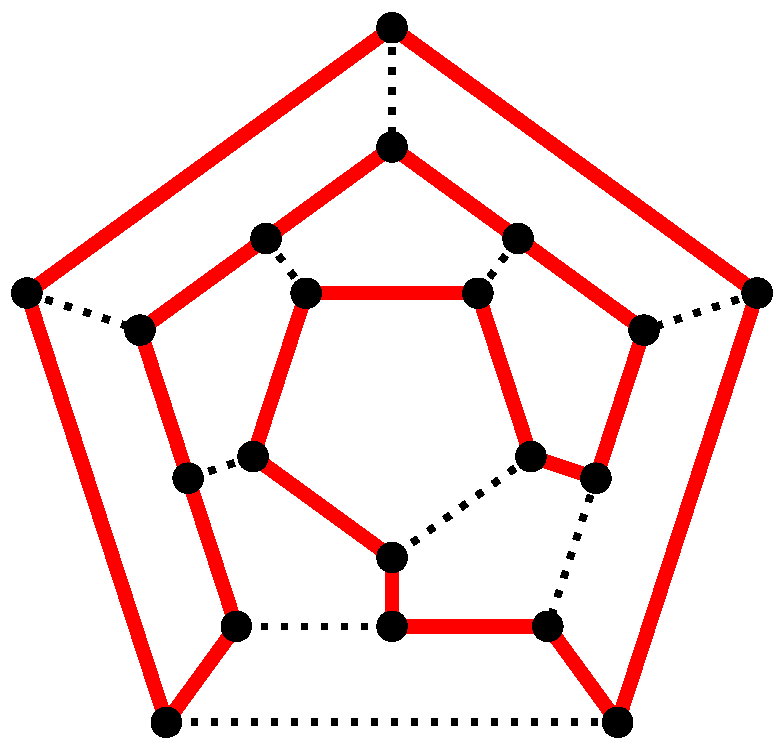
\includegraphics[width=.5\linewidth]{img/Hamiltonian_path.pdf}
\end{center}

\vspace{-.5\baselineskip} %
Ce livret contient 3 activités débranchées pour explorer la base de
l'informatique

\medskip
\centerline{\large\textit{Qu'est ce qu'un algorithme?}}

\bigskip
\centerline{  
\includegraphics[width=.9\linewidth]{img/logo_SMN.pdf}}

\begin{spacing}{.5}
{\tiny Vous pouvez copier, modifier et diffuser librement ce document,\\
  à condition de laisser ces mêmes droits à vos lecteurs (licence CC-BY-SA).}
\end{spacing}
%%%%%%%%%%%%%%%%%%%%%%%%%%%%%%%%%%%%%%%%%%%%%%%%%%%%%%%%%%%%%%%%%%%%%%%%%%%%
%%%%%%%%%%%%%%%%%%%%%%%%%%%%%%%%%%%%%%%%%%%%%%%%%%%%%%%%%%%%%%%%%%%%%%%%%%%%
%%%%%%%%%%%%%%%%%%%%%%%%%%%%%%%%%%%%%%%%%%%%%%%%%%%%%%%%%%%%%%%%%%%%%%%%%%%%
\section*{Le jeu de Nim}

\vspace{-.5\baselineskip}
Ce premier jeu se joue à deux joueurs.\\
On dispose de 16 objets quelconques.\\
Chacun à son tour prend 1, 2 ou 3 objets.\\
\textbf{But du jeu:} prendre le dernier.

\vspace{-.5\baselineskip}
\subsubsection*{Un algorithme pour gagner}

\vspace{-.5\baselineskip} %
Le joueur n$^o$2 a une \textbf{stratégie gagnante} infaillible: il
s'assure de laisser 12, 8 puis 4 objets à son adversaire.

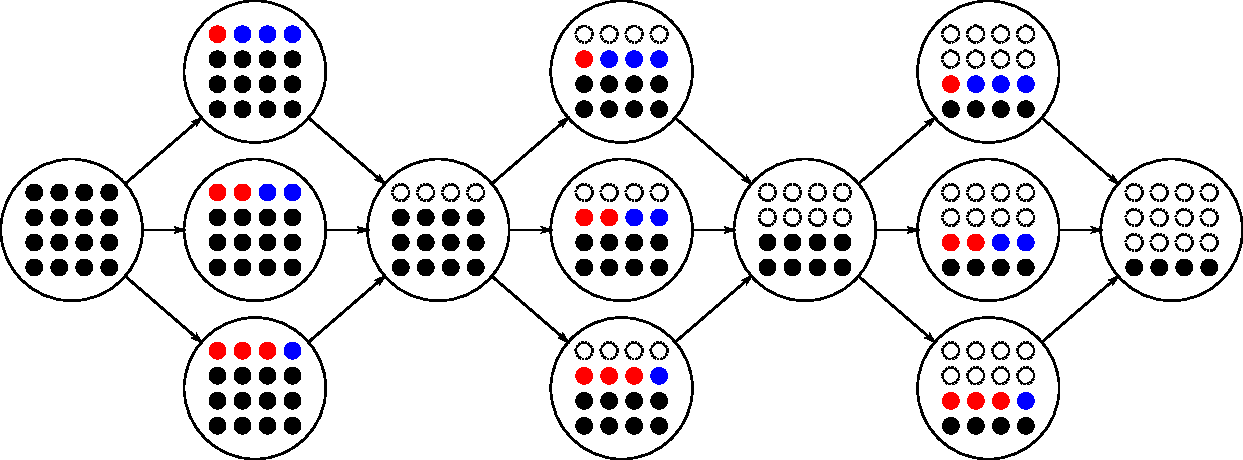
\includegraphics[width=\linewidth]{img/nim16.pdf}

\subsection*{C'est de l'informatique}
\vspace{-.5\baselineskip} %
Les algorithmes sont très importants pour assurer que l'ordinateur
fasse \textbf{à coup sûr} ce que l'on attend de lui.

\newpage
%%%%%%%%%%%%%%%%%%%%%%%%%%%%%%%%%%%%%%%%%%%%%%%%%%%%%%%%%%%%%%%%%%%%%%%%%%%%
%%%%%%%%%%%%%%%%%%%%%%%%%%%%%%%%%%%%%%%%%%%%%%%%%%%%%%%%%%%%%%%%%%%%%%%%%%%%
%%%%%%%%%%%%%%%%%%%%%%%%%%%%%%%%%%%%%%%%%%%%%%%%%%%%%%%%%%%%%%%%%%%%%%%%%%%%
\section*{Le crêpier psycho-rigide}

\vspace{-.5\baselineskip}
Les planchettes sont des crêpes, qu'il faut ranger de la plus grande à
la plus petite.

\smallskip
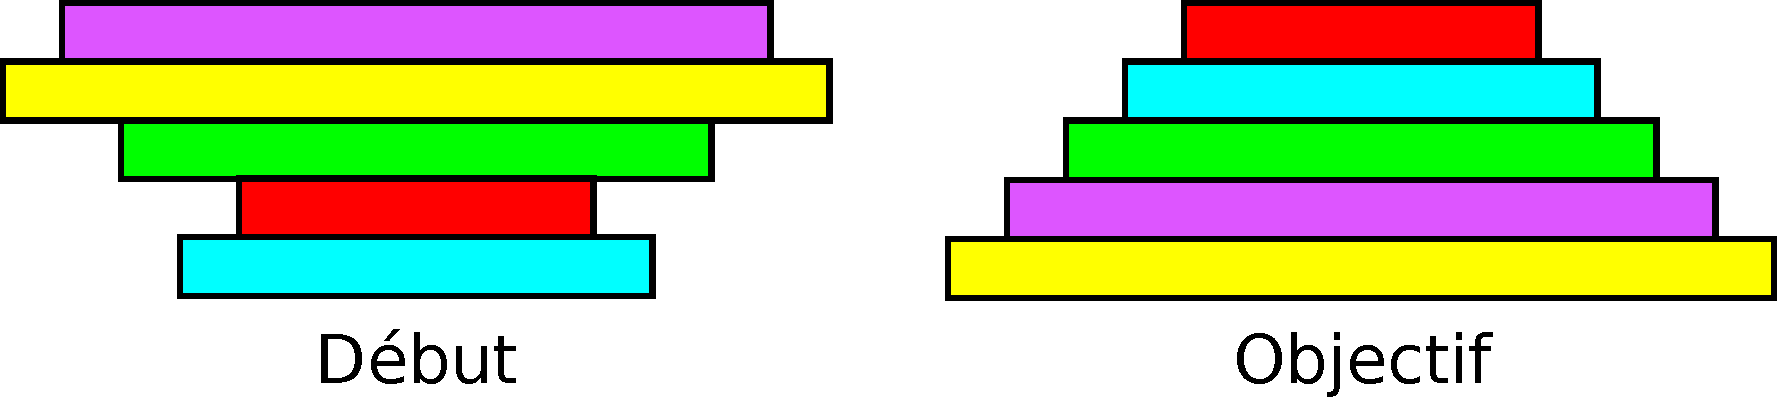
\includegraphics[width=\linewidth]{img/crepes_but-du-jeu.pdf}

À chaque coup, on retourne le haut de la pile (une ou plusieurs crêpes,
d'un bloc).

\smallskip
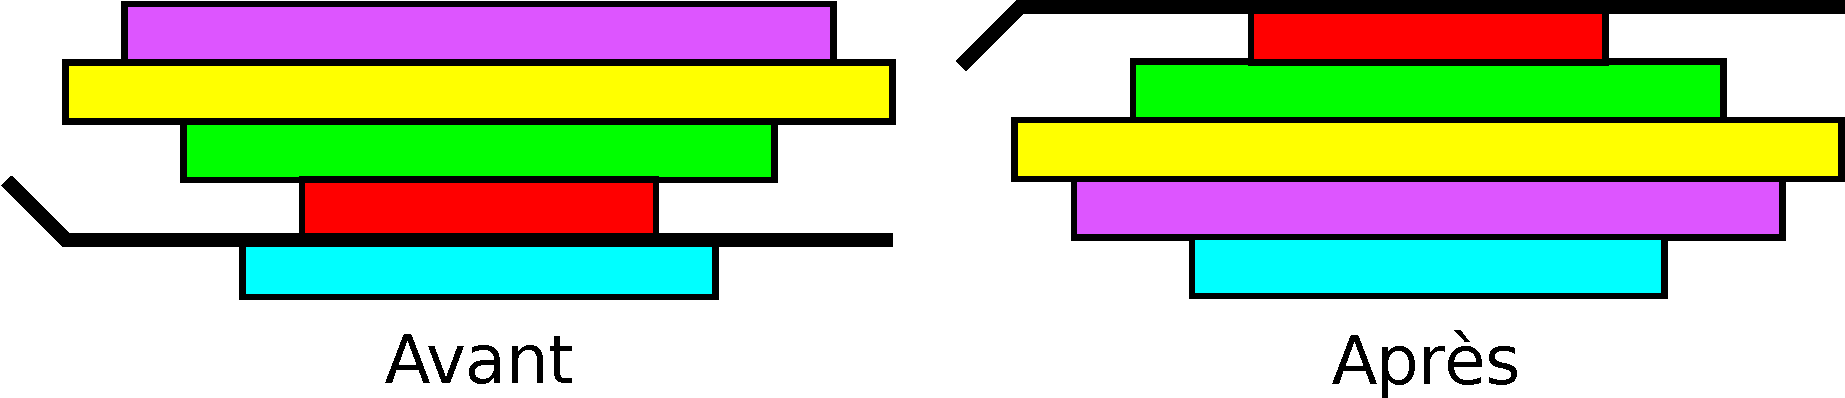
\includegraphics[width=\linewidth]{img/crepes_un-coup.pdf}

\medskip%
On n'a pas le droit de poser des crêpes à coté, ni de soulever celles
du haut pour changer celles au milieu de la pile.

\bigskip%
\textbf{Variante} (plus dure): il faut en plus que la face colorée des
crêpes soit visible.

\newpage
\subsection*{Trouver l'algorithme du crêpier}
\vspace{-.5\baselineskip}

Il faut se fixer des objectifs intermédiaires. Par exemple, placer la
plus grand crêpe tout en bas puis ne plus y toucher.

\smallskip
Est-ce qu'il y a une situation où je sais amener la grande crêpe tout en bas?

\smallskip
Comment faire pour me ramener dans cette situation où je sais ranger la grande crêpe?

\subsection*{C'est de l'informatique}
\vspace{-.5\baselineskip}

Un algorithme, ce n'est pas forcément compliqué. Tout le monde peut en découvrir.

\smallskip
Un ordinateur est très obéissant: il lui faut des instructions
précises et sans ambiguïté.

\vspace{-.5\baselineskip}
\subsection*{Aller plus loin}
\vspace{-.5\baselineskip}
D'autres algorithmes existent pour ce problème. On peut les programmer
avec PLM, l'\textit{exerciseur de l'apprenti programmeur}.\\
{\small\color{blue}\url{http://www.loria.fr/~quinson/PLM/}}

\newpage ~\vfill \centerline{(page 5 vide pour l'instant)} \vfill
\newpage ~\vfill \centerline{(page 6 vide pour l'instant)} \vfill
\newpage ~\vfill \centerline{(page 7 vide pour l'instant)} \vfill
\newpage ~\vfill \centerline{(page 8 vide pour l'instant)} \vfill

\end{document}
